% !TEX root = ../thesis.tex
% \pdfbookmark[0]{Acronyms}{Acronyms}
\chapter{Tools}
There are many tools which make analysing and understaing flaws
of programs very easy. Most of them are not required and work
can be done without them, but they are a good creature comfort
and sholud be used as such.\\\\These tools are used to analyse a 
piece of code and understand its vulnerabilites and also to 
generate payloads to make exploiting them easier.

\section{GDB}
GDB is one of the most importatnt tools. It is one of, if not the 
most importatnt tool for exploiting binaries. It is essentially 
a debugger which allows for dissasmbly of binaries, is also usefull 
for checking the flow of the the binary, and before Ghidra was 
one of the most popular tools to understand the working of a program.
\\\\ It is still used for basic analysis, to check if the exploit 
works, and for initial routing checking. If someone is starting out 
with binary exploitation, then that someone should exclusively use 
GDB till the fundamentals of exploitation done are understood.

\subsection*{Basic Setup}
GDB is usually pre installed on any linux machine. But if it isn't, 
it can be installed using the default package manager ( Like apt or 
pacman ).\\\\There are some extensions for GDB that make it a much 
easier tool to operate with. You can use any number of them to 
make it to your liking, but in the following section, only some 
extensions are used and explained.



\section{radare2}
Radare is a tool which helps in understanding the binary, decompiling 
it and allowing to modify commands on the fly. It is considered one of 
the most difficult tools to master, so much so, that they themselves 
put Figure 6 on their website. I think this can be the Maya of exploiation 
tools.

\begin{figure}
    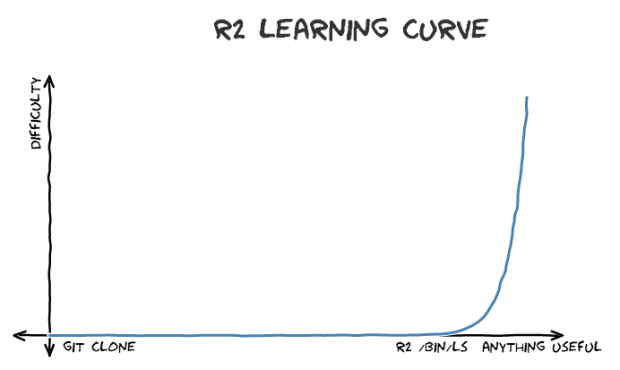
\includegraphics[width = 0.50\textwidth, center]{gfx/radare_learning.png}    
    \caption{Radare Learning Curve}
\end{figure}